\documentclass[a4paper,10pt]{article}
\usepackage{My_math_package}



\title{MATH868C - Several Complex Variables}
\author{Haoran Li}
\date{2018 Fall}

\makeindex[columns=2, title=Index, intoc] % Create the index

\begin{document}\sloppy % reduce overlong words

% Maketitle
\begin{titlepage}
\begin{center}
\vspace*{1cm}
\LARGE
\textbf{MATH868C - Several Complex Variables} \\
\vspace{2cm}
\begin{center}
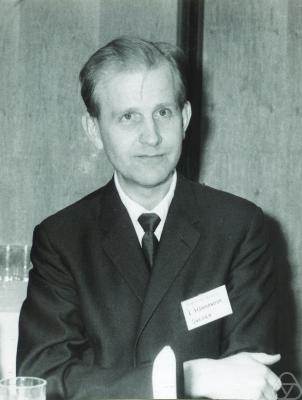
\includegraphics[width=0.5\textwidth]{Pictures/Lars_Hormander.jpg}
\end{center}
\vspace{2cm}
\normalsize
Taught by \texttt{Tam\'as Darvas} \\
Notes taken by \texttt{Haoran Li} \\
2018 Fall \\
\vspace{2cm}
Department of Mathematics\\
University of Maryland\\
\end{center}
\end{titlepage}

\tableofcontents
\newpage

\section{Subharmonic functions}
\subfile{Subharmonic_functions.tex}
\newpage

\section{Cauchy's formula}
\subfile{Cauchy's_formula.tex}
\newpage

\section{Hartogs phenomenon}
\subfile{Hartogs_phenomenon.tex}
\newpage

\section{Plurisubharmonicity}
\subfile{Plurisubharmonicity.tex}
\newpage

\section{Homeworks}
\subfile{Homeworks/Homeworks-main.tex}
\newpage

\begin{thebibliography}{}

\bibitem{An Introduction to Complex Analysis in Several Variables - Hormander} 
\textit{An Introduction to Complex Analysis in Several Variables} - Lars H\"ormander

\bibitem{Complex Analytic and Differential Geometry - Demailly} 
\textit{Complex Analytic and Differential Geometry} - Jean-Pierre Demailly

\end{thebibliography}

\printindex
\newpage

\end{document}